\documentclass[tikz,border=10pt]{standalone}
\usetikzlibrary{calc}
\begin{document}
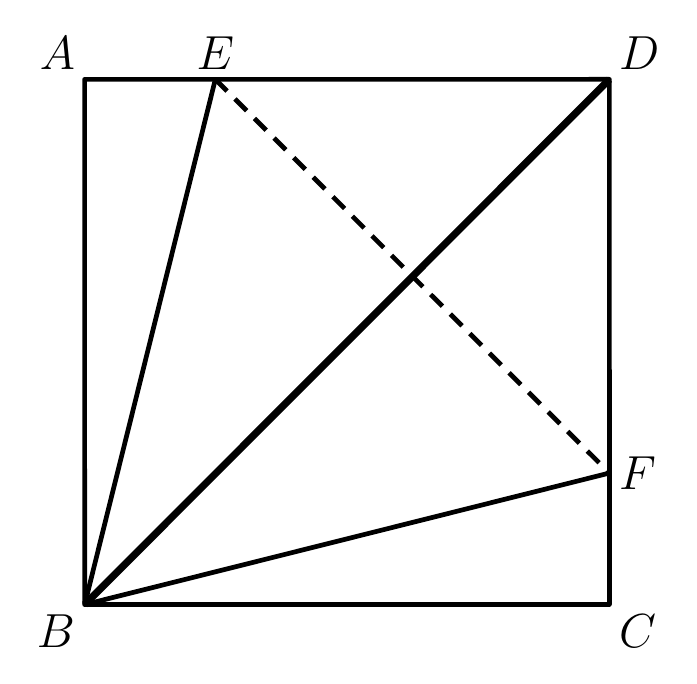
\begin{tikzpicture}[line join=round]
% Named coordinates (cm). Scale s = 0.021164 cm/px, centre (238.5,235.5) px, y flipped.
\coordinate (A) at (-3.3325091645605753,3.3361292056999923);   % px (81,78)
\coordinate (B) at (-3.332116137134793,-3.3338816472015687);  % px (81,393)
\coordinate (C) at (3.3322024728155104,-3.3334889551886726);   % px (396,393)
\coordinate (D) at (3.3318094453897276,3.336521897712888);    % px (396,78)
\coordinate (E) at (-1.6724906864114966,3.336227021551211);   % px (159.4,77.7), on top edge
\coordinate (F) at (3.332104069901626,-1.6635075225738507);   % px (396,314), on right edge

% Solid square sides (metric stroke 1.7pt)
\draw[line width=1.7pt] (A) -- (B) -- (C) -- (D) -- cycle;

% Thick solid diagonal BD (unchanged)
\draw[line width=2.6pt] (B) -- (D);

% Solid segments BE and BF, now 1.7pt to match square sides
\draw[line width=1.7pt] (B) -- (E);
\draw[line width=1.7pt] (B) -- (F);

% Dashed segment EF (unchanged)
\draw[line width=1.7pt, dash pattern=on 6pt off 4pt] (E) -- (F);

% Labels (font from STYLE METRICS plain math labels)
\node[above left, font=\fontsize{17}{20.4}\selectfont] at (A) {$A$};
\node[below left, font=\fontsize{17}{20.4}\selectfont] at (B) {$B$};
\node[below right, font=\fontsize{17}{20.4}\selectfont] at (C) {$C$};
\node[above right, font=\fontsize{17}{20.4}\selectfont] at (D) {$D$};
\node[above, font=\fontsize{17}{20.4}\selectfont] at (E) {$E$};
\node[right, font=\fontsize{17}{20.4}\selectfont] at (F) {$F$};
\end{tikzpicture}
\end{document}
% GEOAGENT_REPAIR_V1 c18a466396f54661 33da818c0a8a51a247d1642588c4980006430179aec9f33a62331b51694014df
